%% 附录A 模板排版功能示例

\chapter{模板排版功能示例}\label{chap:appendix-demo}

本附录展示华侨大学学位论文\LaTeX{}模板所支持的各种排版功能。每个示例模块均标注了学校格式规范的对应要求，供使用者对照检查。

格式规范来源：《华侨大学研究生学位论文的基本要求及撰写格式（2026年第一、二批毕业研究生使用）》。

%% ============================================================
\section{章节标题层级}\label{sec:demo-sections}
%% ============================================================

学校规范对各级标题的要求如下（见规范表2.4）：

\begin{itemize}
  \item \textbf{章标题}：章序号采用"第X章"形式（阿拉伯数字），章序号与章名之间空一个汉字符。黑体三号字，居中书写，单倍行距，段前空24磅，段后空18磅。
  \item \textbf{一级节标题}：序号如"2.1"，黑体四号（14pt）字，居左书写，行距固定值20磅，段前空24磅，段后空6磅。
  \item \textbf{二级节标题}：序号如"2.1.1"，黑体小四号（12pt）字，居左书写，行距固定值20磅，段前空12磅，段后空6磅。
  \item \textbf{三级节标题}：序号如"2.1.2.1"，黑体小四号（12pt）字，居左书写，行距固定值20磅，段前空12磅，段后空6磅。
\end{itemize}

节的层次最多不超过三级。编号深度设置为 \verb|secnumdepth=3|。

\subsection{二级节标题示例}\label{subsec:demo-subsection}

这是一个二级节标题（subsection）的示例。

\subsubsection{三级节标题示例}\label{subsubsec:demo-subsubsection}

这是一个三级节标题（subsubsection）的示例，编号格式为"A.1.1.1"。目录中仅显示到二级节标题，由 \verb|tocdepth=2| 控制。

%% ============================================================
\section{正文段落格式}\label{sec:demo-text}
%% ============================================================

学校规范要求（见规范2.7.5）：

\begin{itemize}
  \item 采用小四号（12pt）字，汉字用宋体，英文用 Times New Roman 体。
  \item 两端对齐书写，段落首行左缩进2个汉字符。
  \item 行距为固定值20磅，段前空0磅，段后空0磅。
\end{itemize}

以下为长文本排版示例：

域适应是迁移学习中的一个重要研究方向，旨在解决训练数据（源域）和测试数据（目标域）分布不一致的问题。在医学图像分析领域，域偏移现象尤为普遍：不同医疗机构使用的设备型号、扫描参数和成像协议可能存在差异，导致图像的灰度分布、对比度和噪声水平各不相同。这种域间差异严重影响了深度学习模型的泛化能力，限制了其在临床实践中的广泛应用。

无监督域适应方法利用源域标注数据和目标域无标注数据，通过缩小两个域之间的分布差异来提升模型在目标域上的性能。常见的技术路线包括：基于对抗学习的方法通过域判别器迫使编码器学习域不变表示；基于图像翻译的方法通过跨域风格迁移消除视觉差异；基于自训练的方法利用伪标签进行迭代学习。近年来，无源域适应进一步放松了对源域数据的访问限制，仅需源域预训练模型和目标域无标注数据即可实现域适应，在数据隐私保护日益严格的医疗场景中具有重要的实际价值。

%% ============================================================
\section{图片}\label{sec:demo-figures}
%% ============================================================

学校规范要求（见规范表2.5）：

\begin{itemize}
  \item 图按章编号，如"图2.1"（附录中为"图A.1"）。
  \item 图序与图名置于图的\textbf{下方}，采用宋体11pt字居中书写，段前空6磅，段后空12磅，单倍行距。
  \item 图序与图名文字之间空一个汉字符宽度。
  \item 如果一个图由两个或两个以上分图组成，各分图分别以(a)、(b)、(c)……作为图序，并须有分图名。
  \item 图中标注的文字采用9\textasciitilde10.5pt，坐标轴题名、描述性词语须采用中文。
\end{itemize}

\subsection{单图示例}\label{subsec:demo-single-fig}

使用 \verb|figure| 环境插入图片。如图~\ref{fig:demo-single} 所示为一个用TikZ直接绘制的单图示例。交叉引用写法为 \verb|图~\ref{fig:xxx}|。

\begin{figure}[htbp]
  \centering
  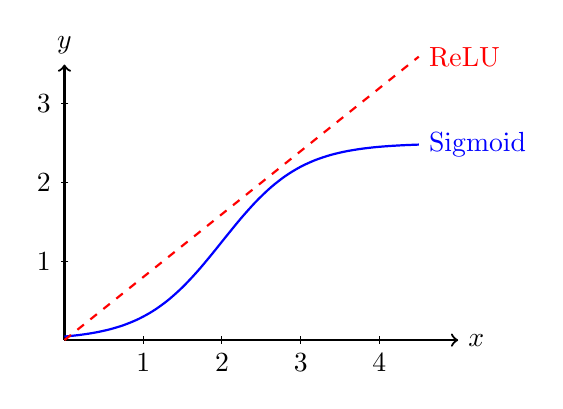
\begin{tikzpicture}
    \draw[thick, ->] (0,0) -- (5,0) node[right] {$x$};
    \draw[thick, ->] (0,0) -- (0,3.5) node[above] {$y$};
    \draw[domain=0:4.5, smooth, thick, blue] plot (\x, {2.5*1/(1+exp(-2*(\x-2)))}) node[right] {Sigmoid};
    \draw[domain=0:4.5, smooth, thick, red, dashed] plot (\x, {max(0, 0.8*\x)}) node[right] {ReLU};
    \foreach \x in {1,2,3,4} \draw (\x, 0.05) -- (\x, -0.05) node[below] {\x};
    \foreach \y in {1,2,3} \draw (0.05, \y) -- (-0.05, \y) node[left] {\y};
  \end{tikzpicture}
  \caption{常见激活函数对比示意图}
  \label{fig:demo-single}
\end{figure}

\subsection{子图示例}\label{subsec:demo-subfigure}

使用 \verb|subcaption| 宏包的 \verb|subfigure| 环境实现分图排列，各分图编号为(a)、(b)等。如图~\ref{fig:demo-subfig} 所示，其中图~\ref{fig:demo-sub-a} 为输入图像示意，图~\ref{fig:demo-sub-b} 为分割标注示意。

\begin{figure}[htbp]
  \centering
  \begin{subfigure}[b]{0.45\textwidth}
    \centering
    \begin{tikzpicture}[scale=0.8]
      \draw[fill=blue!20] (0,0) rectangle (3,2);
      \draw[fill=red!20] (1,0.5) rectangle (2.5,1.5);
      \node at (1.5,1) {\small ROI};
      \node at (0.5,1.7) {\small 图像};
    \end{tikzpicture}
    \caption{输入图像示意}
    \label{fig:demo-sub-a}
  \end{subfigure}
  \hfill
  \begin{subfigure}[b]{0.45\textwidth}
    \centering
    \begin{tikzpicture}[scale=0.8]
      \draw[fill=gray!20] (0,0) rectangle (3,2);
      \draw[fill=green!40] (1,0.5) rectangle (2.5,1.5);
      \node at (1.5,1) {\small 掩膜};
      \node at (0.5,1.7) {\small 标注};
    \end{tikzpicture}
    \caption{分割标注示意}
    \label{fig:demo-sub-b}
  \end{subfigure}
  \caption{医学图像分割子图排列示例}
  \label{fig:demo-subfig}
\end{figure}

%% ============================================================
\section{表格}\label{sec:demo-tables}
%% ============================================================

学校规范要求（见规范表2.5）：

\begin{itemize}
  \item 表按章编号，如"表3.1"（附录中为"表A.1"）。
  \item 表序与表名置于表的\textbf{上方}，采用宋体11pt字居中书写，段前空12磅，段后空6磅，单倍行距。
  \item 表序与表名文字之间空一个汉字符。
  \item 建议采用三线表：上、下边线为单直线，线粗1.5磅；第三条线（表头下方）为单直线，线粗1磅。
  \item 表单元格中的文字采用11pt宋体字，单倍行距，段前空3磅，段后空3磅。
\end{itemize}

\subsection{三线表示例}\label{subsec:demo-booktabs}

使用 \verb|booktabs| 宏包的 \verb|\toprule|、\verb|\midrule|、\verb|\bottomrule| 绘制三线表。如表~\ref{tab:demo-threeline} 所示。

\begin{table}[htbp]
  \centering
  \caption{不同方法的性能比较}
  \label{tab:demo-threeline}
  \begin{tabular}{lccc}
    \toprule
    方法 & DSC (\%) & ASSD (mm) & 参数量 (M) \\
    \midrule
    Method A & 85.32 & 2.14 & 12.5 \\
    Method B & 87.61 & 1.86 & 15.3 \\
    Method C & 89.15 & 1.52 & 18.7 \\
    Ours     & \textbf{91.24} & \textbf{1.23} & 16.2 \\
    \bottomrule
  \end{tabular}
\end{table}

\subsection{多行合并表格示例}\label{subsec:demo-multirow}

使用 \verb|multirow| 和 \verb|\multicolumn| 实现行列合并。使用 \verb|\cmidrule| 绘制局部分隔线。如表~\ref{tab:demo-multirow} 所示。

\begin{table}[htbp]
  \centering
  \caption{消融实验结果}
  \label{tab:demo-multirow}
  \begin{tabular}{clcc}
    \toprule
    \multirow{2}{*}{数据集} & \multirow{2}{*}{方法} & \multicolumn{2}{c}{评价指标} \\
    \cmidrule(lr){3-4}
     & & DSC (\%) & ASSD (mm) \\
    \midrule
    \multirow{3}{*}{Dataset A} & Baseline & 82.10 & 3.05 \\
     & +Module 1 & 85.40 & 2.31 \\
     & +Module 1\&2 & 88.70 & 1.68 \\
    \midrule
    \multirow{3}{*}{Dataset B} & Baseline & 79.50 & 3.42 \\
     & +Module 1 & 83.20 & 2.65 \\
     & +Module 1\&2 & 86.90 & 1.91 \\
    \bottomrule
  \end{tabular}
\end{table}

%% ============================================================
\section{公式}\label{sec:demo-equations}
%% ============================================================

学校规范要求（见规范表2.5）：

\begin{itemize}
  \item 表达式按章编号，用括号括起来置于右边行末，如"式（1.2）"（附录中为"式（A.1）"）。
  \item 表达式应另起行书写，采用与正文相同的字号。
  \item 表达式行的行距为单倍行距，段前空6磅，段后空6磅。
  \item 本模板的公式编号使用中文全角括号"（）"，如（A.1）。
\end{itemize}

\subsection{行内公式}\label{subsec:demo-inline-eq}

行内公式使用 \verb|$...$| 排版，嵌入正文段落中。例如，交叉熵损失函数定义为$\mathcal{L}_{\text{CE}} = -\sum_{c=1}^{C} y_c \log \hat{p}_c$，其中$C$为类别数。Dice系数的取值范围为$[0, 1]$。

\subsection{行间公式}\label{subsec:demo-display-eq}

行间公式使用 \verb|equation| 环境，自动编号并添加全角括号。例如Softmax函数：
\begin{equation}\label{eq:demo-softmax}
  \sigma(\mathbf{z})_i = \frac{e^{z_i}}{\sum_{j=1}^{K} e^{z_j}}, \quad i = 1, 2, \ldots, K
\end{equation}

交叉引用写法为 \verb|式（\ref{eq:xxx}）|。如式（\ref{eq:demo-softmax}）将任意实数向量映射为概率分布。

多行对齐公式使用 \verb|align| 环境，按等号对齐，每行独立编号：
\begin{align}
  \mathcal{L}_{\text{total}} &= \mathcal{L}_{\text{seg}} + \lambda_1 \mathcal{L}_{\text{adv}} + \lambda_2 \mathcal{L}_{\text{rec}} \label{eq:demo-total} \\
  \mathcal{L}_{\text{seg}} &= \frac{1}{2} \mathcal{L}_{\text{CE}} + \frac{1}{2} \mathcal{L}_{\text{Dice}} \label{eq:demo-seg} \\
  \mathcal{L}_{\text{rec}} &= \frac{1}{|\Omega|} \sum_{v \in \Omega} |x(v) - \hat{x}(v)| \label{eq:demo-rec}
\end{align}

如式（\ref{eq:demo-total}）--（\ref{eq:demo-rec}）所示，总损失由分割损失、对抗损失和重建损失三部分组成。

%% ============================================================
\section{算法伪代码}\label{sec:demo-algorithm}
%% ============================================================

使用 \verb|algorithm| 浮动体环境和 \verb|algorithmic| 环境排版伪代码。算法标题格式与图表标题一致。如算法~\ref{alg:demo-training} 所示。

\begin{algorithm}[htbp]
  \caption{自训练域适应算法}
  \label{alg:demo-training}
  \begin{algorithmic}[1]
    \REQUIRE 源域预训练模型 $f_\theta$，目标域无标注数据 $\mathcal{D}_T = \{\mathbf{x}_j^t\}_{j=1}^{N_t}$
    \ENSURE 适应后的模型参数 $\theta^*$
    \STATE 初始化教师模型 $\theta_T \leftarrow \theta$，学生模型 $\theta_S \leftarrow \theta$
    \FOR{$\text{epoch} = 1$ \TO $E$}
      \FOR{each mini-batch $\mathcal{B} \subset \mathcal{D}_T$}
        \STATE 用教师模型生成伪标签：$\hat{y} = \arg\max f_{\theta_T}(\mathbf{x}^t)$
        \STATE 计算分割损失：$\mathcal{L} = \mathcal{L}_{\text{CE}}(f_{\theta_S}(\mathbf{x}^t), \hat{y})$
        \STATE 更新学生模型：$\theta_S \leftarrow \theta_S - \eta \nabla_{\theta_S} \mathcal{L}$
        \STATE 更新教师模型（EMA）：$\theta_T \leftarrow \alpha \theta_T + (1-\alpha) \theta_S$
      \ENDFOR
    \ENDFOR
    \RETURN $\theta^* = \theta_T$
  \end{algorithmic}
\end{algorithm}

%% ============================================================
\section{参考文献引用}\label{sec:demo-citations}
%% ============================================================

学校规范要求（见规范2.7.7）：

\begin{itemize}
  \item 引文标注遵照GB/T 7714-2015，采用顺序编码制，文献依照引用顺序编码。
  \item 正文中引用文献须在引用处标示序号，文献序号采用"上标"格式。
  \item 本模板使用 \verb|natbib| 宏包配合 \verb|gbt7714-numerical| 样式，启用 \verb|sort&compress| 选项，连续编号自动压缩为区间形式。
\end{itemize}

单篇引用示例：Ronneberger等人\cite{ronneberger2015unet}提出了U-Net网络。

多篇引用示例：深度学习在医学图像分析中得到了广泛应用\cite{ronneberger2015unet,goodfellow2014gan,he2016resnet}。

连续编号压缩示例（sort\&compress）：相关研究见文献\cite{ronneberger2015unet,goodfellow2014gan,he2016resnet,pan2010survey,lecun2015deeplearning,zhao2019review}。

%% ============================================================
\section{脚注}\label{sec:demo-footnotes}
%% ============================================================

学校规范要求（见规范2.7.8）：

\begin{itemize}
  \item 脚注序号采用 \ding{172}\ding{173}\ding{174} 样式的数字编排，以"上标"字体标示在正文句末。
  \item 脚注序号按页编排，不同页的脚注序号不需要连续。
  \item 脚注内容采用宋体小五号字（9pt），两端对齐，单倍行距，段前段后均空0磅。
  \item 序号与脚注内容文字之间空半个汉字符，悬挂缩进1.5个中文字符。
\end{itemize}

这是第一个脚注的示例\footnote{这是一个脚注示例，用于补充正文中的说明性信息。脚注采用宋体小五号字，悬挂缩进1.5字符，序号与内容间空半个汉字符。}。这是第二个脚注\footnote{脚注序号按页编排，每页重新开始编号，不同页之间不连续。}。

%% ============================================================
\section{列表}\label{sec:demo-lists}
%% ============================================================

列表环境通过 \verb|enumitem| 宏包设置为紧凑格式（无额外间距）。

\subsection{有序列表}\label{subsec:demo-ordered}

使用中文括号编号"（1）（2）（3）"风格：
\begin{enumerate}[label=（\arabic*）]
  \item 提出了一种基于量化特征对齐的无监督域适应分割方法；
  \item 提出了一种基于群体模板先验与课程学习的无源域适应自训练方法；
  \item 在前列腺跨模态MRI数据集上验证了所提方法的有效性。
\end{enumerate}

\subsection{无序列表}\label{subsec:demo-unordered}

域适应方法的主要类别：
\begin{itemize}
  \item 图像空间适应方法
  \item 特征空间适应方法
  \item 自训练方法
  \item 对比学习方法
\end{itemize}

%% ============================================================
\section{页眉页脚与页码}\label{sec:demo-header-footer}
%% ============================================================

学校规范要求（见规范1.5）：

\begin{itemize}
  \item \textbf{页眉}：偶数页内容为"华侨大学博士（或硕士）学位论文"，奇数页内容为当前一级标题名称。各部分首页也要有页眉。宋体五号字居中书写，页眉下横线为单横线。
  \item \textbf{页码}：封面、答辩决议、声明页不加页码；从中文摘要到目录用大写罗马数字"I、II、III……"；从第1章到论文结束用阿拉伯数字"1、2、3……"。页码置于页面下部居中，Times New Roman五号字。
  \item \textbf{页面设置}：A4纸，页边距上3.8cm、下3.8cm、左3.2cm、右3.2cm，页眉距边界2.8cm，页脚距边界2.8cm。
\end{itemize}

以上设置均在 \verb|hquThesis.cls| 中通过 \verb|geometry|、\verb|fancyhdr| 宏包自动实现，使用者无需手动调整。

%% ============================================================
\section{目录格式}\label{sec:demo-toc}
%% ============================================================

学校规范要求（见规范2.5）：

\begin{itemize}
  \item 标题"目录"采用黑体三号字，居中书写，单倍行距，段前空24磅，段后空18磅。
  \item 目录列至二级节标题（如2.2.5）即可。
  \item 章标题行：黑体小四号字，固定行距20磅，段前空6磅，段后0磅，居左书写。
  \item 一级节标题行：宋体小四号字，行距固定值20磅，左缩进1个汉字符。
  \item 二级节标题行：宋体小四号字，行距固定值20磅，左缩进2个汉字符。
\end{itemize}

以上设置通过 \verb|hquThesis.cls| 中的 \verb|titletoc| 宏包自动实现。
